\documentclass[a4paper,utf8]{article}
\usepackage[heading,fancyhdr]{ctex}
\usepackage{amsmath,amssymb,geometry,lastpage,ulem}
\usepackage{array,tabularx,graphicx}
\geometry{
    top=25.4mm, 
    left=30mm, 
    right=30mm, 
    bottom=35mm,
    headsep=5.9mm,
}
\ctexset{
    section = {format+=\raggedright}
}
\newcommand{\expinfo}[5]{
    {\zihao{-3}\bfseries\songti
    实验名称:\uline{\hfill\mbox{#1}\hfill} \\[2.9mm]
    学\quad 号:\uline{\makebox[25mm]{#2}}\hfill
    姓\quad 名:\uline{\makebox[25mm]{#3}}\hfill
    班\quad 级:\uline{\makebox[25mm]{#4}} \\[2.9mm]
    合作者:\uline{\makebox[25mm]{无}}\enspace~
    桌\quad号:\uline{\makebox[25mm]{}}\hfill\mbox{}\\[2.9mm]
    指导教师:\uline{\makebox[30mm]{#5}}\hfill\mbox{} \\[2.9mm]
    实验日期:\uline{\makebox[30mm]{}}\hfill\mbox{} \\[58.7mm]
    }
}%\expinfo{实验名称}{学号}{姓名}{班级}{指导教师}
\pagestyle{fancy}
\fancyhf{} \fancyhead[C]{材料科学基础实验} \fancyfoot[C]{\thepage~/~\pageref{LastPage}}
\begin{document}
\begin{center}
    {\mbox{}\\[7em]\zihao{2}\bfseries\songti%
    材料科学基础实验报告}\\[34mm]
    \expinfo{实验三 碳钢退火、正火后的组织观察与硬度分析}{22301070}{杨雨燃}{22材物}{杨玉华}
\end{center}
\newpage
\section*{【实验目的】}
    \begin{enumerate}
        \item 了解碳钢的退火、正火过程。
        \item 观察和研究碳钢经不同退火处理、正火处理后显微组织的特点,分析热处理工艺对其组织与硬度的影响,并了解退火、正火的应用领域。
    \end{enumerate}   
\section*{【实验原理】}%简单描述,含必要的公式和附图;
\textbf{(一) 退火}

退火处理是将工件加热到适当温度并保温, 然后进行缓慢冷却的热处理方法。其目的是使工件内部组织达到或接近平衡状态,获得良好的工艺性能和使用性能,或者为进一步淬火过程作组织准备。

1.完全退火(加热至 $A_3+30 \sim 50$°C)
主要用于消除毛坯件中的魏氏组织、带状组织等组织缺陷,调整硬度、改善切削加工性能。

2.不完全退火(加热至 $A_1 \sim A_3$°C)
主要目的是降低硬度、改善切削加工性、消除内应力;
特点为加热温度低,消耗热能少,降低工艺成本。

3.球化退火(加热至$A_1+20$°C)
降低硬度、改善切削加工性、改善组织、提高塑性等。

4.去应力退火(加热到相变点 $A_1$ 以下的某一温度)
消除由于冷热加工所产生的残余应力。

5.扩散退火(加热至 $A_3$ 或 $A_{cm}$+150$\sim $300°C)
又称均匀化退火,用于合金钢锭和铸件。以消除枝晶偏析,使成分均匀化。

\textbf{(二)正火}

正火处理与一般退火的不同之处在于试样在空气中以稍大的冷却速度中进行冷却。由于正火冷却速度较快,过冷度较大因而发生伪共析组织转变,使组织中珠光体量增多,且珠光体的层片厚度减小,故得到精细结构。
这时所获得的组织为索氏体 S 或屈氏体 T 属珠光体类型,是铁素体和渗碳体的混合物。用于消除过共析钢中的网状二次渗碳体,为进一步的球化退火作好组织准备。

\textbf{(三)退火与正火加热温度选择}

\begin{center}
    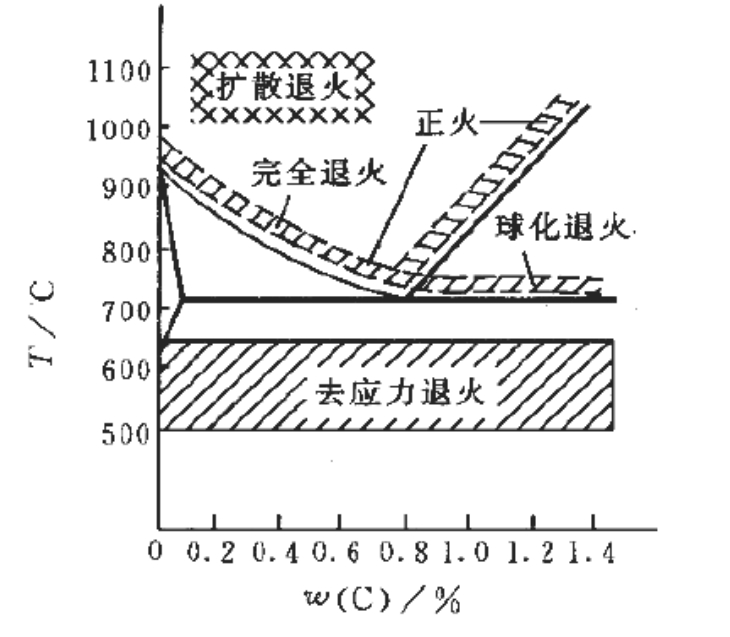
\includegraphics[width=200pt]{1.png}
\end{center}

上图是退火和正火的加热温度范围图。

\textbf{(四)退火与正火保温时间的确定 }

 τ = KD

式中,K为加热系数,一般K=1.5$\sim$2.0min/mm;D为工件有效尺寸。装炉量不大时可以使用此式。


\textbf{(五)显微组织的观察}

若白色网状组织比较粗大,且粗细不均匀,并且还能清楚看到网状组织中存在黑色细而均匀的线条(即晶界),则可以判断该组织为铁素体;若白色网状组织很细很均匀,则可判断为网状二次渗碳体。

亚共析碳钢一般采用完全退火,经退火后可得接近于平衡状态的组织,即铁
素体加珠光体。T12钢经球化退火后组织为球状珠光体。
二次渗碳体和珠光体中的渗碳体都呈球状(或粒状),左图。45钢正火组织
为铁素体+索氏体如右图。
\begin{center}
    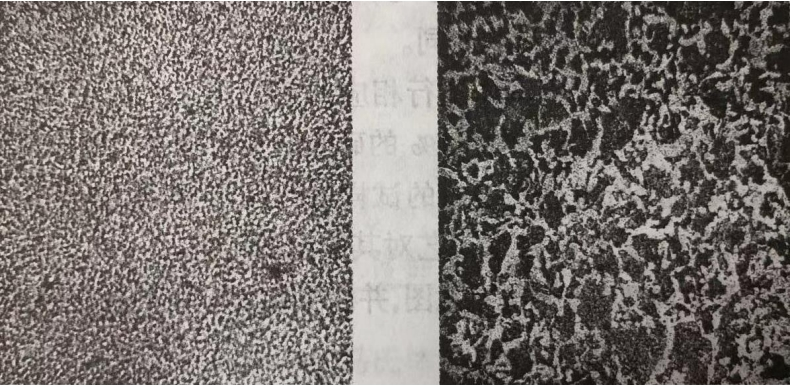
\includegraphics[width=350pt]{2.png}
\end{center}
\section*{【实验仪器】}%规格及参数
箱式电阻加热炉,洛氏硬度计,砂纸,抛光机,金相显微镜。热处理试样:
45钢及T12钢。
\section*{【实验过程】}%简述主要过程和实验内容
1、4人一组,45钢(2个)、T8(1个)及T12钢(1个),(对应下表中相应的热处理工艺方法)

\begin{center}
    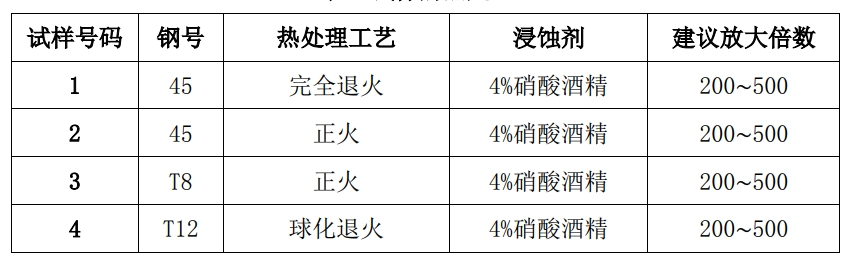
\includegraphics[width=350pt]{3.png}
\end{center}

2、制定热处理工艺参数,可参考以下工艺参数。

① 45钢完全退火工艺:加热温度为860 ± 10℃,根据试样有效尺寸计算保温
时间,保温后炉冷到500℃左右出炉空冷。

② 45钢正火工艺:加热温度为860 ± 10℃,根据试样有效尺寸计算保温时
间,保温后出炉空冷。

③ T8钢正火工艺:加热温度为820 ± 10℃,根据试样有效尺寸计算保温时间,
保温后出炉空冷。

④ T12钢球化退火工艺:加热温度为760 ± 10℃,根据试样有效尺寸计算保
温时间(约40分钟),保温后随炉冷却到680℃保温40分钟,随后炉冷到500℃出
炉空冷。

3、利用硬度计对所有热处理后的试样进行硬度测试,每个试样至少三个试验点,再取一个平均值,分析热处理工艺对其硬度的影响。按照下表选用硬度计。(硬度测试须在金相磨制观
察前完成)

\begin{center}
    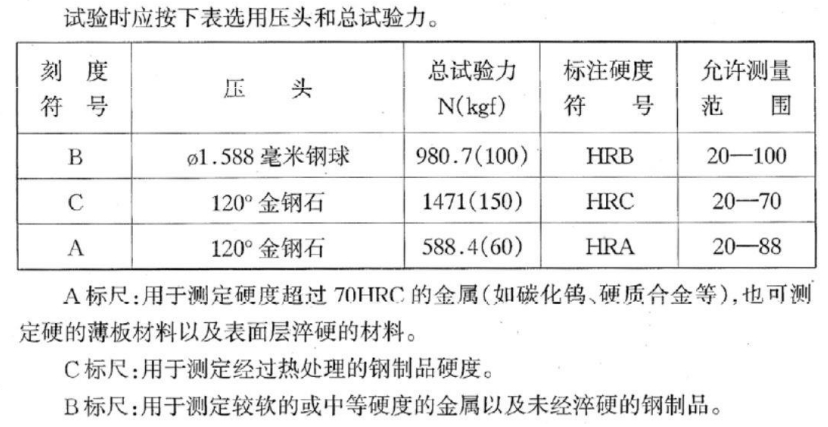
\includegraphics[width=350pt]{4.png}
\end{center}


4、根据拟定的热处理工艺对试样进行相应的热处理工艺处理,然后利用金相砂
纸对热处理后的试样进行磨制、抛光,并用4\%的硝酸酒精进行腐蚀制得金相试样。
利用金相显微镜对其进行显微组织观察,分析热处理工艺对其组织的影响。

5、实验结束后,汇总各小组实验数据,根据实验数据分析冷却方法对碳钢性能(硬度)的影响,并阐明硬度变化的原因。

\newpage

\section*{【实验数据】}

\begin{table}[!ht]\centering
    \caption{不同热处理试样的硬度}
    \extrarowheight=11pt
    \begin{tabularx}{\textwidth}{|c|X|X|X|X|}\hline
        材料及热处理状态 & \multicolumn{3}{c}{测得硬度数据} & \hfil 平均值 \hfil \\[10pt] \hline
        45 钢经完全退火 &  &  &  &  \\[10pt] \hline
        45 钢经正火 &  &  &  &  \\[10pt] \hline
        T8 钢经正火 &  &  &  &  \\[10pt] \hline
        T12 钢经球化退火 &  &  &  &  \\[10pt] \hline
    \end{tabularx}
\end{table}

\end{document}